% --------------------------------------------------------------------------
% This is a LaTeX template for a University of Idaho Master's thesis.
% It uses a custom document class file, UIdahoMastersThesis
% The class and template adhere to the formatting guidelines established by UI College of Graduate Studies (CoGS) as of 2016.
% That being said, DOUBLE CHECK everything, I'm not perfect, and this isn't either. 
% I highly recommend getting it reviewed by the Writing Center and CoGS BEFORE you're finished writing. Seriously.
% --------------------------------------------------------------------------
% Author   Christopher Goes
% Email    goesc@acm.org    (Alternate: goes8945@alumni.uidaho.edu)
% --------------------------------------------------------------------------
% This template (and my thesis!) would not be possible without the work of these awesome people.
%     - Matthew Brown, CS       For sharing his thesis and all the neat hacks it had
%     - Cara Leatherman, CoGS   For template improvements
%     - Chris Zeoli, CoGS       For the original UI CoGS template
% --------------------------------------------------------------------------

% This includes the magical class file with the formatting. ** DO NOT REPLACE THIS. Everything WILL break. **
\documentclass{UIdahoMastersThesis}

% --------------------------------------------------------------------------
% Packages (the class file already imports several. Importing twice usually doesn't hurt, just keep in mind for debugging)
%\usepackage{apacite}

\usepackage[latin1]{inputenc}
\usepackage[T1]{fontenc}
\usepackage[printonlyused]{acronym} % Use [nolist,nohyperlinks] to not write list of acronyms and not put hyperlinks to entries in list.
% ** Add any packages you want to use here **

%\usepackage{tgbonum}
\usepackage{lmodern}

\usepackage{hyphenat}
\usepackage{siunitx}

%--- for \enquote ---
\usepackage[english]{babel}
\usepackage{csquotes}
%Beginning of the interresting part
\DeclareQuoteStyle[american]{english}
	{\itshape\textquotedblleft}
    [\textquotedblleft]
    {\textquotedblright}
    [0.05em]
    {\textquoteleft}
    {\textquoteright}
%End of the interresting part

\usepackage{graphicx} % for figures {figure}
\usepackage{float}
\usepackage[font=small,labelfont=bf]{caption}

\usepackage{epigraph}
%-- special markup to fix up epigraph style
\usepackage{etoolbox}
\makeatletter
\newlength\epitextskip
\pretocmd{\@epitext}{\em}{}{} %this makes the text entry italics
\apptocmd{\@epitext}{\em}{}{}
\patchcmd{\epigraph}{\@epitext{#1}\\}{\@epitext{#1}\\[\epitextskip]}{}{}
\makeatother

\setlength\epigraphrule{0.5pt}
\setlength\epitextskip{1ex}
\setlength\epigraphwidth{.72\textwidth}

%-- make \quote font smaller----
\usepackage{relsize,etoolbox}% http://ctan.org/pkg/{relsize,etoolbox}
\AtBeginEnvironment{quote}{\smaller}% Step font down one size relative to current font.

\makeatletter  % ** DO NOT REMOVE THIS ** (Actually, remove it, compile, and enjoy the stream of errors. Its beautiful :) )


% --------------------------------------------------------------------------
% Thesis Information
\title{Ecstatic [X]Reality}
%\subtitle{Expanding Consciousness with Cross Reality}
\author{Zeth duBois}
\thesisdegree{Master of Science}  % e.g Master of Science, Master of Engineering, etc.
\major{Integrated Architecture and Design}  % e.g Computer Science, Computer Engineering, etc.
\advisor{Roger Lew, Ph.D.}  % Make sure title of names matches CoGS format requirements!
\cmone{John William Anderson}  % First committee member (Alphabetical order by last name, if I recall correctly)
\cmtwo{Alistair Smith, Ph.D.}  % Second committee member
\deptadmin{John William Anderson}  % Department administrator or chair
\graddate{May, 2020}  % Graduation date, e.g May, 2017
% --------------------------------------------------------------------------


% Line spacing. The University of Idaho requires thesis formatting to be 1.5-2.0. In LaTeX 1.3=1.5, 1.6=2.0.
\linespread{1.6}

% Defines section counter for frontmatter. This way section number does not appear in the TOC for frontmatter sections
\setcounter{secnumdepth}{0}

% Sets what level of sections show up in the table of contents. 0 = sections, 1 = subsections, 2 = subsubsections, etc.
\setcounter{tocdepth}{1}


% Configure the PDF output (Most of this is optional, it just adds metadata to the PDF)
\usepackage[% pdftex
pdfauthor=\author,
pdftitle=\title,
pdfsubject={Example subject},
pdfkeywords={keyword1;keyword2;etc},
pdfproducer={ShareLatex},  % e.g ShareLatex
pdfcreator={pdflatex},
pdfprintscaling={AppDefault}]
{hyperref}

% Configure hyperlinks
\hypersetup{
	colorlinks=true, %set true if you want colored links
	linktoc=all,     %set to all if you want both sections and subsections linked
	linkcolor=black,  %choose some color if you want links to stand out
	citecolor=black,
	urlcolor=black,
}

% Changes default indenting in list of figures to 0 
%\makeatletter
\renewcommand*\l@figure{\@dottedtocline{1}{0em}{2.3em}}% Default: 1.5em/2.3em
\let\l@table\l@figure
%\makeatother

% Where to look for images 
% (https://en.wikibooks.org/wiki/LaTeX/Importing_Graphics#Graphics_storage)
\graphicspath{ {./Figures/} }

% Uncomment to set default style for Listings to be code (Code style is defined in .cls file)
% \lstset{style=code}


% -------------------------------------------------------------------------
\begin{document}

\frontmatter

\titleformat{\chapter}[block]{\scshape\LARGE}{\centering\chaptertitlename\  \thechapter:}{1ex}{\centering}{}
	\titlespacing{\chapter}{0pt}{-40pt}{20pt}

\titleformat{\section}[hang]{\scshape\Large}{\thesection}{1ex}{}
    \titlespacing{\section}{0pt}{0pt}{10pt}
	%\titlespacing*{\section}{0pt}{-50pt}{40pt}

\titleformat{\subsection}[hang]{\scshape\large}{\thesubsection}{1ex}{}
    \titlespacing{\subsection}{0pt}{0pt}{10pt}
	%\titlespacing*{\subsection}{0pt}{-50pt}{40pt}


% -------------------------------------------------------------------------
% -- Title Page --
\thesistitlepage


% --------------------------------------------------------------------------
% -- Authorization to Submit Thesis --
\frontmattersection{Authorization to Submit Thesis}
\authorizationpage
\newpage


% --------------------------------------------------------------------------
% -- Abstract --
\frontmattersection{Abstract}
\begin{center}
	{\LARGE\textsc{Abstract}}
\end{center}

For tens of thousands of years, cultures have practiced ecstatic rituals. With the rise of organized religion and the rational scientific revolutions, knowledge of practices and techniques faded into myth. Ecstasy can be described as a highly charged emotional state, that is both volatile and short-lived, presenting the conscious mind with inexplicable mental visions. Contemporary western culture eschews the value of ecstatic ritual, in favor of rational problem-solving. The ecstatic experience is personal, unfathomable, and the only outward signs of its features are in the accounts of subjects relating their experiences. The ephemeral subjectivity of ecstasy presents numerous barriers for the formal investigation of the transformation of ecstasy, in both scientific credo and societal acceptance. 

A person may use non-invasive mental techniques of meditation, prayer, trance, and the like, to achieve an ecstatic state of mind. Ingesting psychoactive compounds can also lead to ecstasy. Until the 20th century, these processes have been primarily held to be the domain of spiritual exploration. With parallel advances of both inorganic and organic chemistry, scientists discovered psychoactive chemicals inherent in plants reacted in the brain in unforeseen ways. Further exploration of natural compounds and fully human-made laboratory chemicals revealed the existence of neurotransmitters, demonstrating that the experience of consciousness can be directed by temporarily altering brain neurochemistry.

The ecstatic experience relates to a state of perception of self in a world of sensation. It is conceivable that that deviation from ordinary frames of reference, as shown by the recordings in the stories of shamans, religious practitioners, yogis, and scientific experimentation, is central to the benefits inherited from an altered state of mind. Evidence has shown that ecstatic ritual well-conceived can have lasting therapeutic effects for mood disorders, assist in overcoming chemical addictions, and enhance overall peace of mind.


Accepting that ecstasy is a personal voyage wherein the individual reimagines itself in an altered world, is it also possible to direct the development of strictly external sensations to assist in the development of similar outcomes? This paper will explore the use of \textit{\ac{XR}} to craft uniquely adapted multisensory experiences. \ac{XR} is a technique that makes use of technologies of virtualization---sensory simulation of a believable world---and interaction with adaptive data processing, to include any accessible global data and real-time characteristics of the user. Accessing ecstasy with the aid of \ac{XR}, \textit{\ac{EXR}}  offers hitherto unreachable features of altered state consciousness. Chief among them is the opportunity to be observed by third parties---which is to say, empirical, and to some degree, reproducible. \ac{EXR} can be simultaneously a door to spiritual discovery, and a research tool into the workings of the conscious mind.


\newpage


% --------------------------------------------------------------------------
% -- Acknowledgements --
 \frontmattersection{Acknowledgments}
 \begin{center}
 	{\LARGE\textsc{Acknowledgments}}
 \end{center}
 
Your acknowledgments.

\newpage


% --------------------------------------------------------------------------
% -- Dedication --
% \frontmattersection{Dedication}
% \vspace*{\fill}
% \begin{center}
%   {\LARGE\textsc{Dedication}}
   
   
% ***  Your dedication. This section is optional, per the handbook. ***
% \end{center}
% \vspace{\fill}
% \newpage


% --------------------------------------------------------------------------
% -- Table of Contents --
\frontmattersection{Table of Contents}
\tableofcontents
\newpage


% --------------------------------------------------------------------------
% -- List of Tables --
% \frontmattersection{List of Tables}
% \listoftables
% \newpage


% --------------------------------------------------------------------------
% -- List of Figures --
\frontmattersection{List of Figures}
\listoffigures
\newpage


% --------------------------------------------------------------------------
% -- List of Code Listings --
% \frontmattersection{List of Code Listings}
% \lstlistoflistings
% \newpage


% --------------------------------------------------------------------------
% -- List of Acronyms --
% This is useful for those in fields with an excessive amount of acronyms, 
\frontmattersection{List of Acronyms}
\begin{center}
	{\LARGE\textsc{List of Acronyms}}
\end{center}

% Use acronyms in a consistent manner and without spelling mistakes
%   \acf{cogs}  Full definition of acronym
%   \ac{cogs}   Regular usage (does the stuff [between braces])
\begin{acronym}[fMRI]  % Passing an acronym as argument makes other acronyms align with it. This is usually the longest acronym.
	\acro{AR}[{\textup{AR}}]{Augmented Reality}
	\acro{VR}[{\textup{VR}}]{Virtual Reality}
	\acro{XR}[{\textup{XR}}]{Cross Reality}
	\acro{EXR}[{\textup{EXR}}]{Ecstatic Cross Reality}
	\acro{ASC}[{\textup{ASC}}]{Altered State of Consciousness}
	\acrodefplural{ASC}[{\textup{ASC}}]{Altered States of Consciousness}
	\acro{fMRI}[{\textup{fMRI}}]{Functional Magnetic Resonance Imaging}
	\acro{EEG}[{\textup{EEG}}]{Electroencephalography}
    %\acro{vm}[VM]{Virtual Machine}  % Normal version of an acronym. Usage: \ac{vm}
    %\acrodefplural{vm}[VMs]{Virtual Machines}  % Plural version of an acronym. Usage: \acp{vm}
\end{acronym}



% --------------------------------------------------------------------------
\mainmatter  % Starts the content part of the thesis
\setcounter{secnumdepth}{3}  % Sets depth section numbers go to. 
% NOTE !! : There is a bug currently where they will not work at depth of 3, e.g section 1.2.3 will not display, but 1.2 will.




% --------------------------------------------------------------------------
% -- Introduction --
\clearpage
\chapter{Introduction}
\label{Chapter:Introduction}
%\section{A Section}
%\subsection{A Subsection}
%Example of acronym: \ac{cogs}
%Using it again: \ac{cogs}
%Plural one: \acp{vm}

\acresetall  % Use this if you want acronyms to be fully stated upon first use again, such as in new chapters

%\epigraph {The mind is its own place, and in itself can make a heaven of hell, a hell of heaven\ldots}{John Milton, Paradise Lost}

\epigraph {If the words 'life, liberty, and the pursuit of happiness' don't include the right to experiment with your own consciousness, then the Declaration of Independence isn't worth the hemp it was written on.}{Terence McKenna}

\vspace{9mm}

Throughout human social development, people have cultivated techniques for achieving ecstatic states of mind. For tens of thousands of years, cultures have practiced ecstatic rituals by temporarily altering the state of perception. Methods range between physically limiting/shaping access to external stimulation to internally altering neurochemical activity. Characteristics of the first pole resolve to practices of prayer, trance, or meditation, utilizing disciplines or techniques to achieve hard to reach brainwave states that minimize occlusion of extra-sensory perception. In the case of neurochemical alterations, states can be achieved via direct regulations in biochemistry. The most effective of these techniques, in terms of accessibility, intensity, and duration, are those induced by the use of powerful exogenous chemicals that radically alter sensory and cognitive processing in the mind. The effects of the methods across this spectrum have been measured in clinical studies, supporting the claim that neurochemistry, brainwave states, and the resulting neurological data visible in cognitive processing can be temporarily altered \cite{carhart-harris_neural_2012}\cite{michael_r._hagerty_case_2013}.

While the entire range of technique is functional to achieving \textit{\acp{ASC}}, the use of chemicals, characterized as \textit{psychoactive}, or mind-altering drugs, provide the most dramatic and sudden state changes. As we well know, a drug toxicity profile can range from extremely lethal to entirely benign, and a thorough understanding of the risks should precede any use of drugs. It has been well demonstrated that long before the advent of laboratory science, the Controlled Substances Act, and the United Nations Convention on Psychotropic Substances, that many naturally-occurring psychoactive chemicals have toxicities so low, that lethal human doses have yet to be discovered. Tryptamines are biologically safer than Tylenol by several orders of magnitude, and yet they are scheduled as the most restricted substances on Earth. However, despite the inconvenient fact that some sources for these banned chemicals spring up unbidden from the daily landscape, as open-source technology for casual harvesting, the legal status makes not only their collection and use prohibited, but also impedes the opportunity to advance scientific research.

Although psychoactive drugs can be used recreationally, the profound changes to mental state experienced are reputed to induce a type of spiritual voyage not easily dismissed as whimsy. Drugs effective at triggering conscious expansion are termed \textit{entheogen}, Greek for ``becoming divine within,'' when used with this intention. Simultaneously, the same drug used in recreational applications might be colloquially termed \textit{psychedelic}.

Entheogens are useful for establishing \textit{altered states of consciousness}. A mind altered may gain access to unique inspirations and emotional insights, by temporarily disrupting ordinary sensations and perceptions and suspending preconceived notions. This results in radical \textit{disassociation} and \textit{ego-dissolution}. The experience can be so profound that some scientists have suggested that ritualistic ecstasy may have been integral to the development of human consciousness in proto man. The abductive Stoned Ape Hypothesis, advanced by Terence and Dennis McKenna, points out that mutagenic mushrooms discovered in the migrations of early savanna hominids would have had a range of effects on the intrepid ingester, from temporary improvements in visual acuity to full-blown conscious epiphany \cite{mckenna_invisible_1993}.

Supporting evidence that something extraordinary was occurring with early human brains during this portion of the human timeline, is present in the sudden and inexplicable doubling of Homo sapiens' cranial capacity in an unprecedentedly short time. Furthermore, it is well-supported that the development of language, broad advances in tool use, and the clear development of societal hierarchical structures occur at this juncture \cite{mckenna_food_1992}.

As the term entheogen is commonly restricted to describing a class of chemicals, let us reflect on the claim that ecstatic states of mind can be captured through self-induced techniques of meditation or trance. Many veterans of ecstasy claim that it is the state of mind and the intention of the undertaking that establishes the efficacy of the entheogen, not the method used to trigger the effect. Expressed more succinctly, it is the entire journey that evokes divinity within. 

Departing from the default world---then returning. This journey is called ecstasy.


\section{A Case for Ecstasy}
The Oxford English Dictionary defines ecstasy as, ``An emotional or religious frenzy or trance-like state, originally one involving an experience of mystic self-transcendence.'' For colloquial uses, especially hyperbolic ones, ecstasy is likely employed to mean ``extremely happy'' or ``thrilled.'' Etymologically, ecstasy draws from Latin meaning ``to be or stand outside oneself,'' and shares similar lineage with the word existence, ``to cause to stand.''
 
Albert Einstein referred to ecstasy as the ``mystical emotion'' and spoke of it as \enquote{\ldots the finest emotion of which we are capable\ldots}. He credits the inspiration of the mysterious as the source of art and science , and that \enquote{anyone to whom this feeling [ecstasy] is alien, who is no longer capable of wonderment and lives in a state of fear, is a dead man \cite{einstein_science_1930}.}

Einstein's existential sentiment for the contact with ecstasy recalls the autobiographical writings of Edward Abey detailing his nearly monastic assignment as a park ranger in the American desert southwest in the 1960s. In his book Desert Solitaire, he emphasizes the role of joy goes beyond individual utility, suggesting that it is a requisite strategy for survival of the species. 

%\epigraph{``Has joy any survival value in the operations of evolution? I suspect that it does; I suspect that the morose and fearful are doomed to quick extinction. Where there is no joy, there can be no courage; and without courage, all other virtues are useless.''}{Edward Abey, Desert Solitaire}

\begin{quote}
{Has joy any survival value in the operations of evolution? I suspect that it does; I suspect that the morose and fearful are doomed to quick extinction. Where there is no joy, there can be no courage; and without courage, all other virtues are useless.}
\end{quote}


There is no scientific consensus on the cause of emotion, but it is generally held to be an experience generated within the nervous system, establishing a mood or mental state. In 1913, the philosopher and psychologist Moritz Geiger, a member of the Munich phenomenological school, described the nature of emotion as ``occupying the experiential side of consciousness.\cite{mayer-gross_translation:_nodate}''   

Striving to establish practical frameworks, psychologists develop theoretical models to attempt to classify emotional dispositions. One such model is the emotion wheel [Figure\ref{fig:wheel}] developed by Robert Plutchik. The wheel considers eight categorical emotions arranged radially with each bipolar emotion opposed. Concentric rings of the wheel indicate three levels of intensity from mild to intense. Plutchik's wheel arranges stages of serenity with joy arriving in ecstasy.

\begin{figure}[h!]
	\centering
	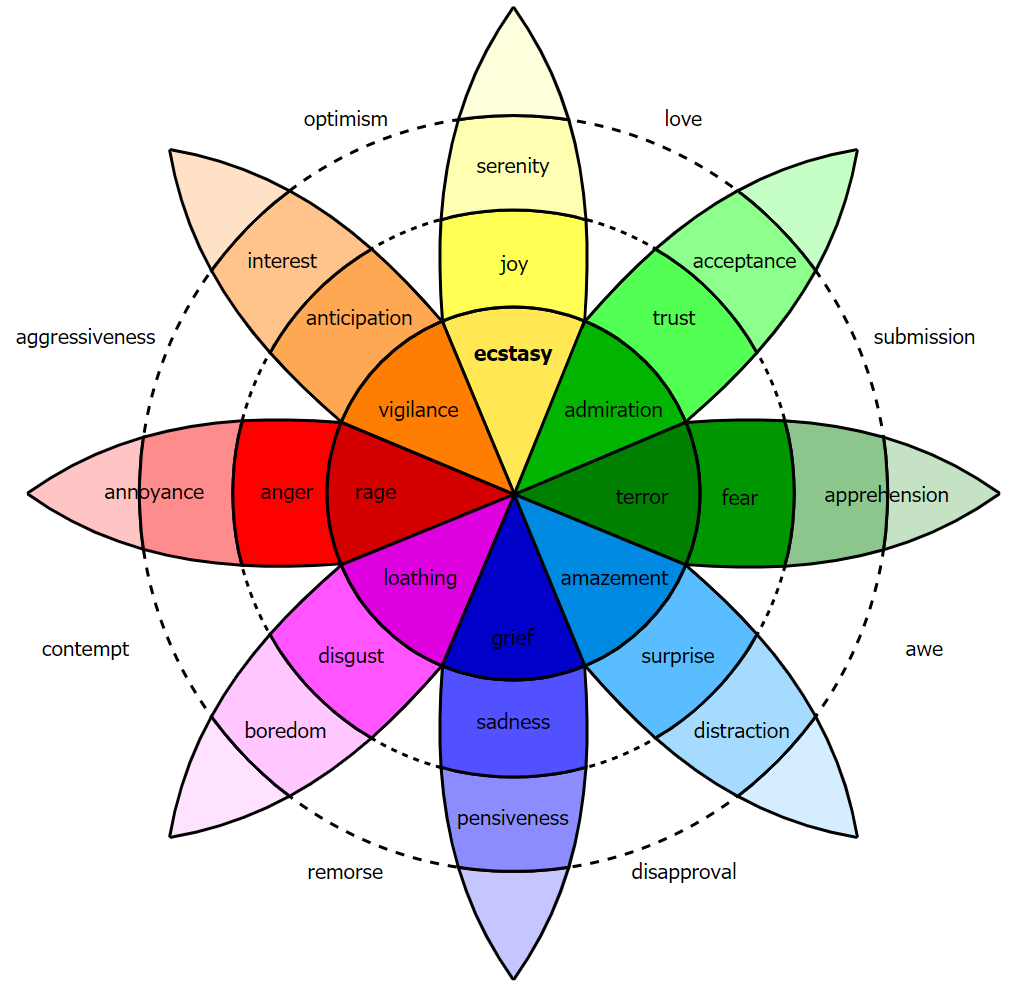
\includegraphics[width=0.72\linewidth]{plutchik_wheel.png}
	\caption{Plutchik Emotion Wheel}
	\label{fig:wheel}
\end{figure}

Similarly, the psychiatrist and philosopher Dr. Neel Burton speaks of the positive feelings of elation as states of euphoria, arriving at the pinnacle of ecstasy. He contends that ecstasy can be a route to epiphany, a sudden and striking realization, or as the Sanskrit root implies, ``a rising wisdom\cite{burton_heaven_2015}.''

This discussion reveals a problematic ambiguity. There is a strong association between ecstasy and happiness or joy, and this misdirects the vital impact of a truly ecstatic experience. The process of becoming ecstatic \emph{can be} joyful, yet drawing, for example, from the emotions in the final ring of the emotional wheel, it is easy to claim that the state of ecstatic mind, as reflected in innumerable accounts, can be equally frightful, grievous, astonishing, loathsome, or fascinating.

Wilhelm Mayer-Gross, a German-born (1889) psychiatrist, wrote his doctoral thesis on the subject of heightened emotion. In his analysis, The Phenomenology of Abnormal Emotions of Happiness, he reviews the literature of self-reported ecstatic experiences, often religious, contrasting with the documentation of psychiatric patients in the throes of mania\cite{mayer-gross_translation:_nodate}.  Mayer-Gross lays out what he considers six basic differences between ecstasy and abnormal happiness. Not to list them all here, the key feature repeated throughout is the observation that ecstasy can swell to displace the phenomena of an external world, to include one's own physical body, whereas happiness retains connection to external objects and phenomena, often as the subject or source of the state of joy itself \cite{beer_nature_2000} . Mayer-Gross refers to this total objective transformation as a dissolution of the self, and this is consistent with the overwhelming majority view from expert scientists, theologians, shaman, and ``ordinary'' people, who contend the overall effect of the ecstatic state is \emph{ego-dissolution}.

As it pertains to the remainder of this writing, the heightened emotional experience of ecstasy is understood as a transformation through exhilaration, of ego-dissolution, and a temporary reprise from the ordinary perceptions of the Self-in-World.

% --------------------------------------------------------------------------
% -- 
\clearpage
\chapter{Expanding Consciousness}
\label{Chapter:Expanding Consciousness}

\emph{\ldots to be or stand outside oneself}\\

As the ecstatic experience relates to an altered state of perception of Self in a world of sensation, and establishing that a departure to said state can be triggered by combinations of experimental doses of nothing (i.e., no exogenous chemicals) and doses of something (e.g., 20 micrograms of DMT), it has been remarked by practitioners, shamans, spiritual leaders, gurus and researchers alike, that psychoactive drugs can be training wheels for the nascent enlightenment achieved through meditation. The directionality of the reference insinuates a preference for meditation, perhaps as a more respectable, if not at least legal, action. The machinations of materialistic cultures being what they are, society prides itself on sober problem solving and is therefore willing to tolerate meditators, while shunning self-medicated drug-users.

\section{Altered States}


The idea of ``self-medicating'' is worthy of further discussion. Scientific advances in biology and organic chemistry triangulate to arrive at contemporary medical practices that condition modern people with the expectation that drugs are medicine for illness. Doctors are specialists who train in the fields of medicine, focusing in select domains or modalities. In a conventional, allopathic practice, they will analyze the complaints of patients, diagnose illness, and then select from a library of formulated solutions to manage the presumed illness, or, more frequently, only treat the symptom. Often the solutions are pharmaceutical---medicine for sick people. These proffered formulations are rarely foods or naturally occurring plants, but instead strictly regulated synthetic drugs. Many pharmaceutical synthetics emulate natural sources that may conceivably be growing in the parking lot or could be sourced from foods known to be high in the active ingredients. However, without a personal and casual relationship with healers, recommending a carefully managed diet, changes in destructive habits, or just common-sense behavior, exposes the system to unverifiable patient compliance, and professional liabilities. With the myriad dangers of our increasingly toxic environments, stressful schedules, and unhealthy habits, it is clear to see how a powerful and impersonal prescription drug culture might inevitably arise as the dominate medical ethos. This is not to say that modern medical science and synthetic pharmaceuticals do not have remarkable life-saving outcomes. Rather, the observation is of the tendency to believe exclusively in the techniques of technology as sacrosanct, approval by trusted authority, forgoing the subtler solutions presented in the natural world, which may be ancient, forgotten, or just too weird.

The converging of these factors has a chilling effect on the public`s will to explore consciousness transformation through psychoactive ritual. Most countries on Earth have made entire classes of psychoactive drugs illegal. The subject matter is effectively taboo. Returning to the academic investigation of consciousness and ecstasy, one must be cautious of falling for the societal tendency of rating the ethics between meditation and [illegal] drug-use. After all, consciousness itself appears to be agnostic to technique, and therefore any judgment regarding practice should remain subjective to individual values (and the aforementioned laws).

Let us observe that deviation from ordinary frames of reference, as shown by the recordings of ecstatic voyagers, may guide participants to beneficial states of mind. Evidence has shown altered mind states can have lasting therapeutic effects for mood disorders, assist in overcoming chemical addictions, and enhance overall peace of mind. With the postulate that the interplay of observing one`s \emph{self} in the world \emph{unexpectedly reframed} leads to ecstatic experiences, what are the specific ways to access ``reframing''---to alter conscious state?

\subsection{affective disorder}

Altering the state of mind is not exclusively a radical, nor is it exclusively an intentional process. Taken literally, altering state occurs at every instance of time as the conscious mind compares a persistent frame of reference from the cumulative past to perceptions of the present moment. Altering state is merely updating the present frame of reference. It is the intensity of alteration that qualifies for distinction as ecstatic. There are examples of ecstatic experiences that occur without the intentional or willing participation of the subject. Such an occurrence might be termed revelation when associated with beneficial foresight, or spiritual fervor. Often in the material and scientific world, spontaneous revelation is dismissed as psychosis.

A 1937 paper by EW Anderson, a clinician at the Cassel psychiatric Hospital in London, documents the study of four patients with a variety of affective disorders who experience bouts of ecstasy \cite{anderson_clinical_1938}. Anderson references E Blueler's Textbook of Psychiatry to define ecstasy as a ``\ldots states of rapture'' in which the outer world is completely interrupted. \enquote{The patients see the heavens open, associate with the saints, hear heavenly music, experience wonderful odours and tastes and indescribable delight of distinct sexual colouring that pervades the entire body.} 

The patients reviewed in the paper were admitted voluntarily and suffered from mild mood or personality afflictions that made them more of a nuisance than a threat to their communities. They moved through various states of psychiatric care before being referred to the hospital. While in the care of the facility, each had one or more ecstatic interludes featuring states of extraordinary calmness, bliss, and disassociation from the normal world. One patient described:

\begin{quote}
{There seemed a trembling vibration over my consciousness, a veil between me and what I should know, as if I were hovering beyond a great mystery. Then a dawning sense of exquisite harmony, without being lifted into the first state of ecstasy\ldots Thought, space, and time dropped away.}
\end{quote}
  
Anderson compared the descriptions to phenomena the late 19th-century psychiatrist RM Bucke called ``cosmic consciousness.'' He concludes that patients' inner tranquility and harmony with the environment was characteristically distinguishable from states of hyper mania. These were not psychotic manic episodes, but inexplicable phases of ecstatic delight.
A more recent paper (1987) about a much older case, neuroscientist D Landsboroug examines biblical references to ecstatic visions ascribed to the apostle Paul. In his letters to the Corinthians, Paul describes ecstatic experiences paired with ``a thorn in his flesh'' that are characterized by depersonalization, a connection to heaven, and auditory revelation [Figure \ref{fig:paul}]. Paul writes:

\begin{quote}
{I simply know that in the body or out of the body this man was caught up to paradise and heard sacred secrets which no human lips can repeat. Of an experience like that, I am prepared to boast\ldots My wealth of visions might have puffed me up, so I was given a thorn in the flesh, an angel of Satan to rack me and keep me from being puffed up.}\cite{bible_new_1984}
\end{quote}

\begin{figure}[h!]
	\centering
	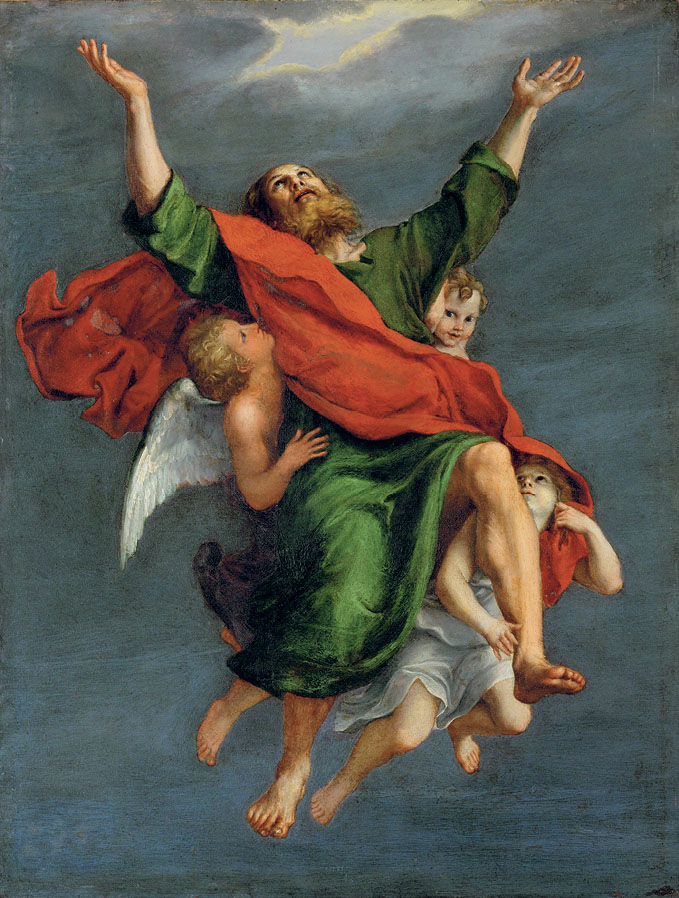
\includegraphics[width=0.63\linewidth]{paul.jpg}
	\caption{Domenichino---The Ecstasy of St Paul, 17th c.}
	\label{fig:paul}
\end{figure}

Paul's ``puffed'' up could mean too prideful, or boastful, from receiving such holy ecstasy. Realizing that he could lose touch with humble piety, he accepts his ``thorn'' as a mortal limitation, a sin physically manifest, retaining his station in the divine order. Landsboroug postulates that both the visions and the thorn were manifestations of temporal lobe epilepsy---a brain disorder that causes seizures and periods of unusual behavior or feelings.

As can be imagined, the debate over the nature of St Paul's thorn has raged for nearly two thousand years. A more recent author, Fyodor Dostoevsky, also had epilepsy. Written in 1868, \emph{The Idiot} tells the story of a young Russian noble returning to St Petersburg following a four-year commitment to a Swiss sanitarium for treatment of his epilepsy. Dostoevsky infuses his character with momentary ecstasy at the brink of each seizure:

\begin{quote}
{\ldots His sensation of being alive and his awareness increased tenfold at those moments, which flashed by like lightning. His mind and heart were flooded by a dazzling light. All his agitation, doubts, and worries seemed composed in a twinkling, culminating in a great calm, full of understanding\ldots}\cite{bible_new_1984}
\end{quote}

Other abnormal cognitive afflictions are known to trigger ecstatic episodes. In the article, The Nature, Causes, and Types of Ecstasy, MD Beer unearths several early 20th-century psychiatry trials reflecting on schizophrenic ecstasy and the resulting elation of manic episodes of disassociation, other-worldly visitations, voices, and hallucinations \cite{beer_nature_2000}

While the involuntary occurrences of affective disorders may occasion an ecstatic response in persons so afflicted, it is also well understood that a voluntary engagement with ecstasy may be actively courted with the practiced discipline of meditation.

\subsection{meditation}

Considering the features of meditation provides further insight into the mechanisms of conscious expanding ecstasy. For the sake of simplicity, meditation discussed here represents the collection of methods focused on changing state of mind though voluntary, sustained, disciplined techniques, to include controlled breathing, chanting, prayer, drumming, dancing, fasting, mindfulness, and silent retreat. Unlike affective disorders or psychoactive drugs, both of which overpower processing behavior in the central nervous system, the key to meditative ecstasy is non-invasive, sustained, and intentional techniques.

Meditation may source a secular credo, but due to the influence of organized religion, and the literary nature of religious scholarship, documentation of meditation/prayer that is of religious or spiritual nature is widely available. The monotheistic lineages of the middle east focus almost exclusively on the historical preservation of divine revelation as received by prophets and apostles. Those references are minimally useful; perhaps best as anthropological clues as to the evolving historical importance of ecstatic ritual at the cultural level.
 
While it is true that monotheists developed a monastic class that spend time in isolated prayer and study, and this undoubtedly qualifies for meditation, the Eastern spiritualities document a wide variety of technique for approaching ecstasy from an individual perspective. Yogic traditions drawing upon the ecstatic forms of meditation are thousands of years old. The Yoga-S\^{u}tra, Bhagavad Gita, Pata\~{n}jali, Vij\~{n}\^{a}nabhairava, and Pratyabhij\~{n}\^{a}hrdayam are classical yoga texts describing ecstatic meditation \cite{waelde_dissociation_2004}.

For example, tradition based on the Vij\~{n}\^{a}nabhairava, a compendium of 112 yoga techniques delivered in verse, guides practitioners to control the mind through disciplined observation. Yogis learn to control state of mind by directing attention away from the senses by, for example, watching the breath, repeating mantras, or evoking visualizations. Verse 104 says to achieve happiness, the yogi should reject identification with his body in favor of the inner Self. 

Lest it appear that The Vij\~{n}\^{a}nabhairava requires a practitioner to deny one part of reality, in preference for another (which the act of perceiving, by process, also must do at every moment) consider a practical example of another verse, which asks the disciple to meditate on the joy of seeing a long-missed friend, so that the mind becomes absorbed in the feeling of joy \cite{singh_vijnanabhairava_2002}.

It is not necessary to rely on the stories of ancient texts and spiritual anecdotes alone. A multi-institutional case study published in 2013 demonstrated that highly trained meditation practitioners are capable of generating and sustaining self-stimulating brain states. Researchers studied a Buddhist concentration technique called jhana that induces \ac{ASC} in a series of eight sequences [Figure \ref{fig:graphjoy}]. The study methods included \ac{fMRI} and \ac{EEG} recordings to observe a Buddhist with 17 years of meditation practice. 

The research concluded five distinct features of the subject's conscious state, (1) external awareness dims, (2) internal verbalizations fade, (3) the sense of personal boundaries is altered, (4) attention is highly focused on the object of meditation, and (5) joy increases to high levels \cite{michael_r._hagerty_case_2013}.

\begin{figure}[h!]
	\centering
	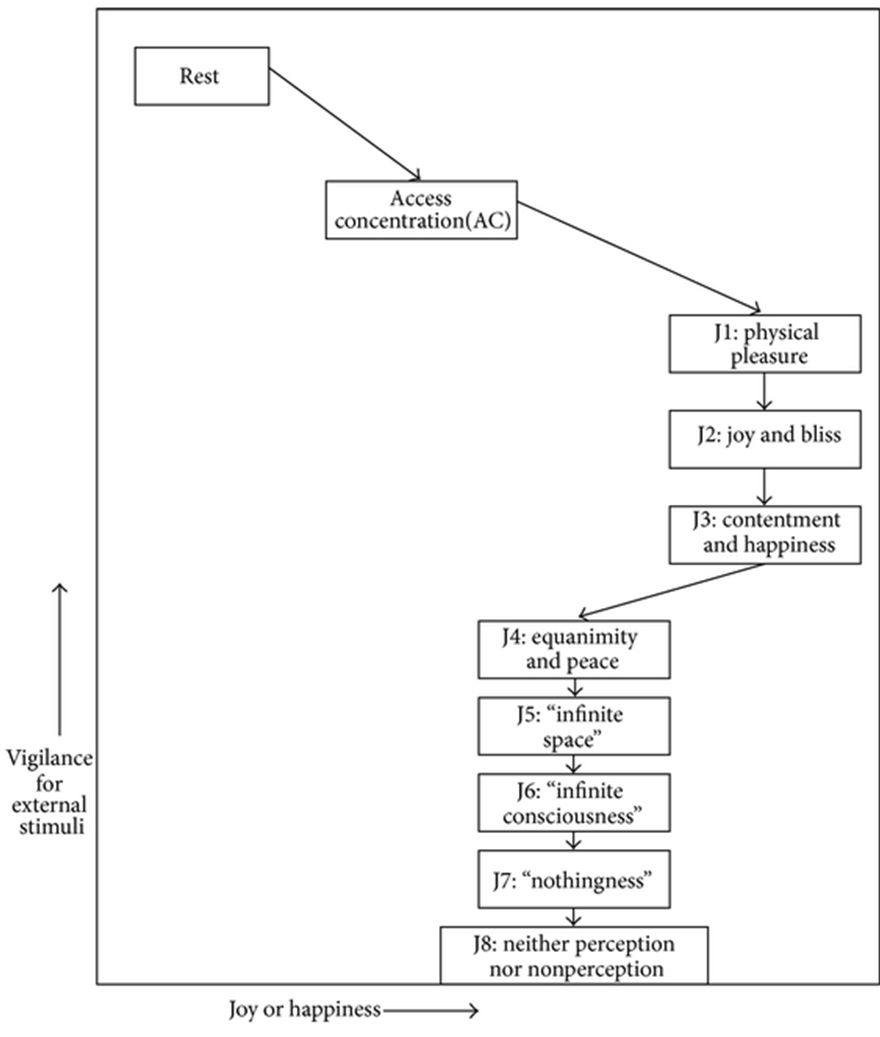
\includegraphics[width=0.63\linewidth]{graph_joy.png}
	\caption{Schematic of the reported experiences in 8 jhanas relative to resting consciousness and concentration on 2 dimensions of interest; \emph{joy or happiness}, and \emph{vigilance for external stimuli}.}
	\label{fig:graphjoy}
\end{figure}



Disciplines like these achieve a practical application, by freeing the individual from undesired effects of worldly phenomenon. Can we consider a skilled meditation practitioner the beneficiary of a sustained ecstatic mind?

Accepting that the disciplined intent of meditation can expand consciousness, let us consider the impact of psychoactive chemicals which portend to achieve analogous effects. 


\subsection{entheogens}

An entheogen is a psychoactive substance used in a spiritual or shamanic context. The term was first coined in 1979 by Ruck, Bigwood, Staples, Ott, and Wasson \cite{ruck_entheogens._1979}, meaning ``becoming the god within'' or ``becoming divine within.''  Entheogens may be directly gathered from natural plant sources, as in mushrooms or cactus flowers; may be brewed from combinations of plants, as in ayahuasca; or may be wholly synthetically derived, like LSD, MDMA, and DMT. Entheogens contain molecules closely related to endogenous neurotransmitters. 

When he was sixty years old, the coincidental Father of LSD addressed the 1966 Worlds of Consciousness Conference in Heidelberg: \enquote{Mystical experiences in [my] childhood, in which Nature was altered in magical ways, had provoked questions concerning the essence of the external, material world, and chemistry was the scientific field which might afford insights into this.} Forty-two years later, Albert Hofmann died at his home in Switzerland, 102 years old.

Dr. Hofmann joined the pharmaceutical-chemical department of Sandoz Laboratories in Basel as a lab chemist. He was working on synthetic derivatives of fungus ergot in 1938 when he developed a series of analogs that failed to produce the intended goals in the laboratory test animals. The formulations were abandoned for five years, until he self-initiated an informal study of one variant, LSD-25, to satisfy a lurking curiosity.
In the handling of the chemicals in the lab on the day of the reboot, Hoffman incidentally absorbed compound from the crystallized tartrate salt product. He sent the following report to the head of the lab, Arthur Stoll:

\begin{quote}
{Last Friday, April 16, 1943, I was forced to interrupt my work in the laboratory in the middle of the afternoon and proceed home, being affected by a remarkable restlessness, combined with a slight dizziness. At home, I lay down and sank into a not unpleasant intoxicated-like condition, characterized by an extremely stimulated imagination. In a dreamlike state, with eyes closed (I found the daylight to be unpleasantly glaring), I perceived an uninterrupted stream of fantastic pictures, extraordinary shapes with intense, kaleidoscopic play of colors. After some two hours, this condition faded away.}\cite{hofmann_lsd:_1980}
\end{quote}

Hoffman had unintentionally become the first person on Earth to have an acid trip. His report to Professor Stoll a few days later demonstrates the well-documented occurrence of \emph{closed-eye hallucinations}. In psychedelic drug culture, hallucinations are frequently a goal of recreational drug users. Fanciful, colorful, elaborate, the styles of visual hallucinations are the hallmark signature of psychedelic art and memorabilia. 

This feature of visual sensation without any light entering the optic system opens inquiry into the nature of consciousness and perception. Famed neurologist Oliver Sacks published his penultimate book, \emph{Hallucinations}, detailing case studies of sensory distortions triggered by fever, injury, drugs, sensory deprivation, exhaustion, and grief. One patient was completely blind, but never-the-less `saw' innumerable visions, including extraordinary specific details of children in brightly colored Eastern clothing, and elves and faeries climbing the sides of her wheelchair. Sacks explains the brain needs not only perceptual input but perceptual change, and that the ``deprivation of normal visual input can stimulate the inner eye'' to produce dreams or hallucinations \cite{sacks_hallucinations_2012}.

Considering these stories of hallucination, whether triggered by bruising the brain falling down a staircase or ingesting \SI{250}{\micro\gram} of LSD, one is hard-pressed to locate within a functional role for a consciousness-expanding ecstatic journey. What use is a fleeting perceptual ``aberration''?

Turning back to the story of Albert Hoffman, three days following his unintended preeminent exposure, he returned to his lab to subject himself to a controlled experiment. Informing a lab assistant of his intentions, he cooked up another batch and measured out what he thought was a safe threshold dose of LSD. Today we know that threshold dosages are in the 10-\SI{20}{\micro\gram} range, with a ``strong'' dose falling between 150-\SI{400}{\micro\gram}. Hoffman took \SI{250}{\micro\gram}.

Within 40 minutes, feelings of anxiety, dizziness, and visual distortions began. He felt in crisis, finding it difficult to speak, but was able to communicate with the assistant that he needed an escort home. On April 17, 1943, Albert Hoffman, under the influence of powerful LSD hallucinations, rode his bicycle home. In his book published in 1979, LSD, My Problem Child he describes the terrifying feelings he endured during the peak of his intoxication, an estimated two hours. Of the following day he writes, 


\begin{quote}
{Exhausted, I then slept, to awake next morning refreshed, with a clear head, though still somewhat tired physically. A sensation of well-being and renewed life flowed through me. Breakfast tasted delicious and gave me extraordinary pleasure. When I later walked out into the garden, in which the sun shone now after a spring rain, everything glistened and sparkled in a fresh light. The world was as if newly created. All my senses vibrated in a condition of highest sensitivity, which persisted for the entire day.}\cite{hofmann_lsd:_1980}
\end{quote}


\begin{figure}%[h!]
  \centering
  \begin{subfigure}[b]{0.4\linewidth}
    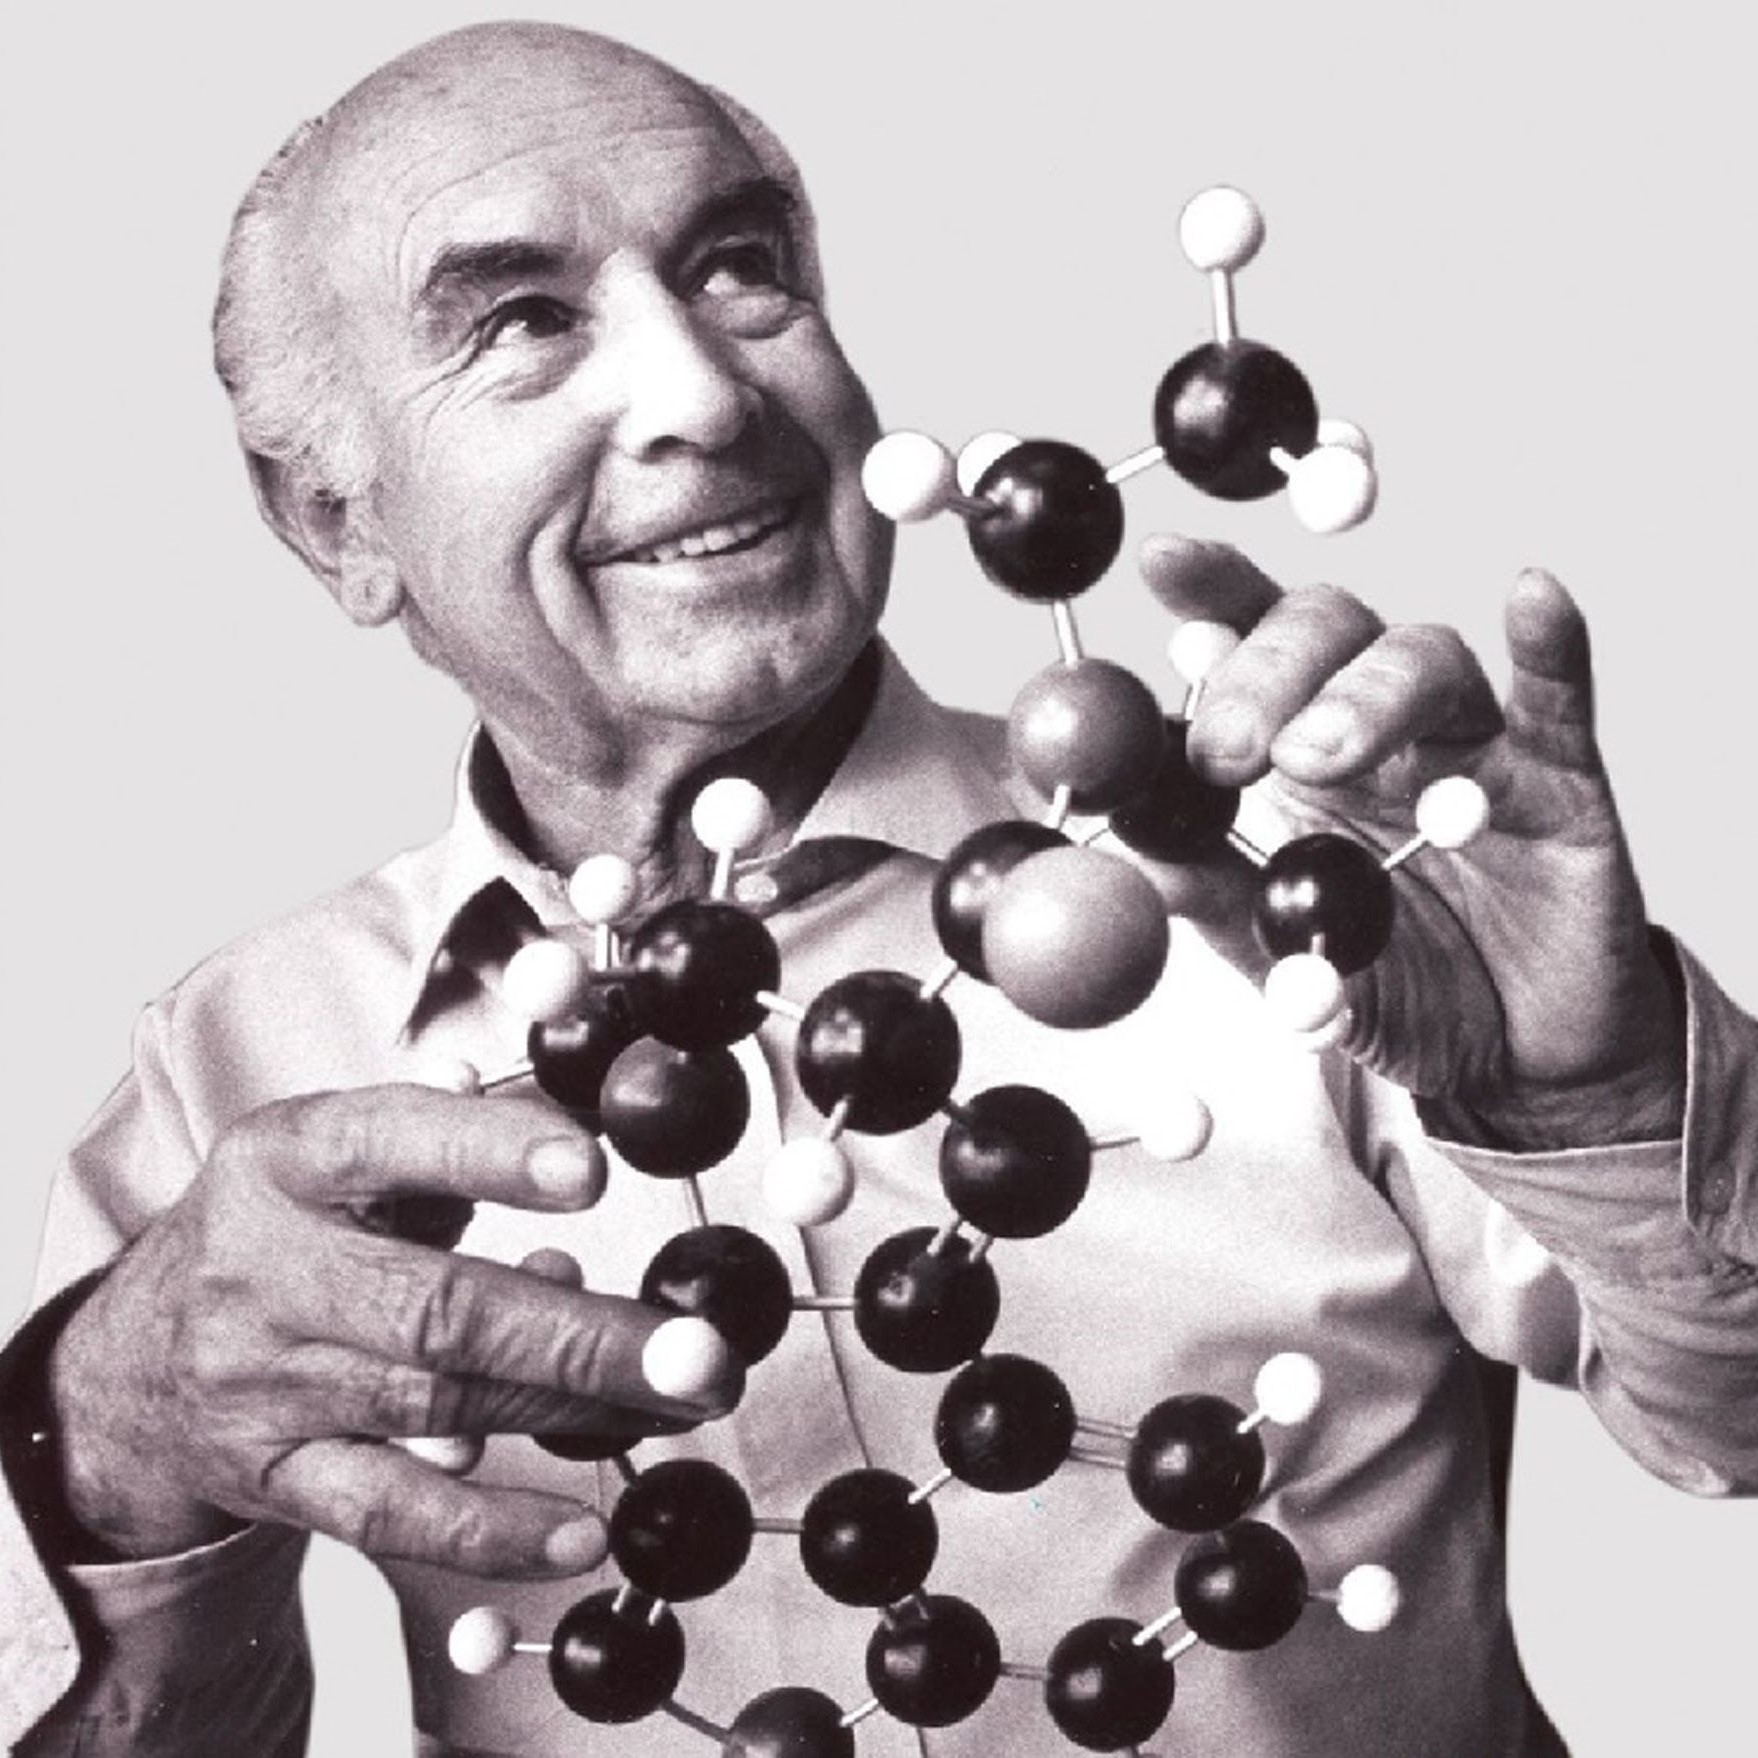
\includegraphics[width=\linewidth]{hofmann_sq.jpg}
    \caption{Dr. Albert Hofmann.}
  \end{subfigure}
  \begin{subfigure}[b]{0.4\linewidth}
    
\includegraphics[width=\linewidth]{bicycle_day.jpg}
    \caption{Bicycle Day - blotter acid}
  \end{subfigure}
  \caption{LSD: Hofmann's \enquote{Problem Child}}
  \label{fig:hofmann}
\end{figure}

The dissidence of comparing fun-loving hallucinating psychedelic trips to the ecstatic experience of ritualistic entheogen trance is reflected on by Ralph Metzner, a pioneer in psychological and cross-cultural studies of consciousness expansion. He is a psychotherapist and professor emeritus at the California Institute of Integral Studies. In his 2017 publication, \emph{Entheogens: Toward an Expanded Worldview for Our Time} he writes,

\begin{quote}
{Whereas the terminology of psychedelics has acquired spurious cultural associations of `tripping,' the historically primal concept of consciousness expansion has two advantages. One, it connects psychedelic drugs with other modes of consciousness expansion, such as meditation and creative visioning; and two, it suggests contrasting comparison with the consciousness contraction involved in concentration and focus.}\cite{metzner_entheogenesis:_2017}
\end{quote}

Whether drug use helps an acolyte to learn the routes to achieve ecstatic meditation, or meditation encourages or works in tandem with entheogenic drug ritual, it is not the focus of this work to take up the position on the primacy of one of these positions over another. Such debate is best left to philosophers, and while we must bear it, legal states who deem it their right to mediate.

\section{A Pscychoactive History}

From the contemporary perspective of Western Civilization, there is little to no expectation for individuals to engage states of ecstasy for beneficial personal growth. Case in point, the drug MDMA invented by German chemists in 1912, would become popularized in the 80s as Ecstasy. Subsequently, the vernacular occurrence of the word has been dominated by the reference to the drug, not the feeling or emotional state for which it was named. To casually verify this assumption, a Google Ngram publication report from 1900-2008 shows the rise in incidence for the term ecstasy to refer to the popular club drug over the emotional state, to eventually rank five times more frequent by the end of the 20th century. [Figure \ref{fig:ngram}]

\begin{figure}[h!]
	\centering
	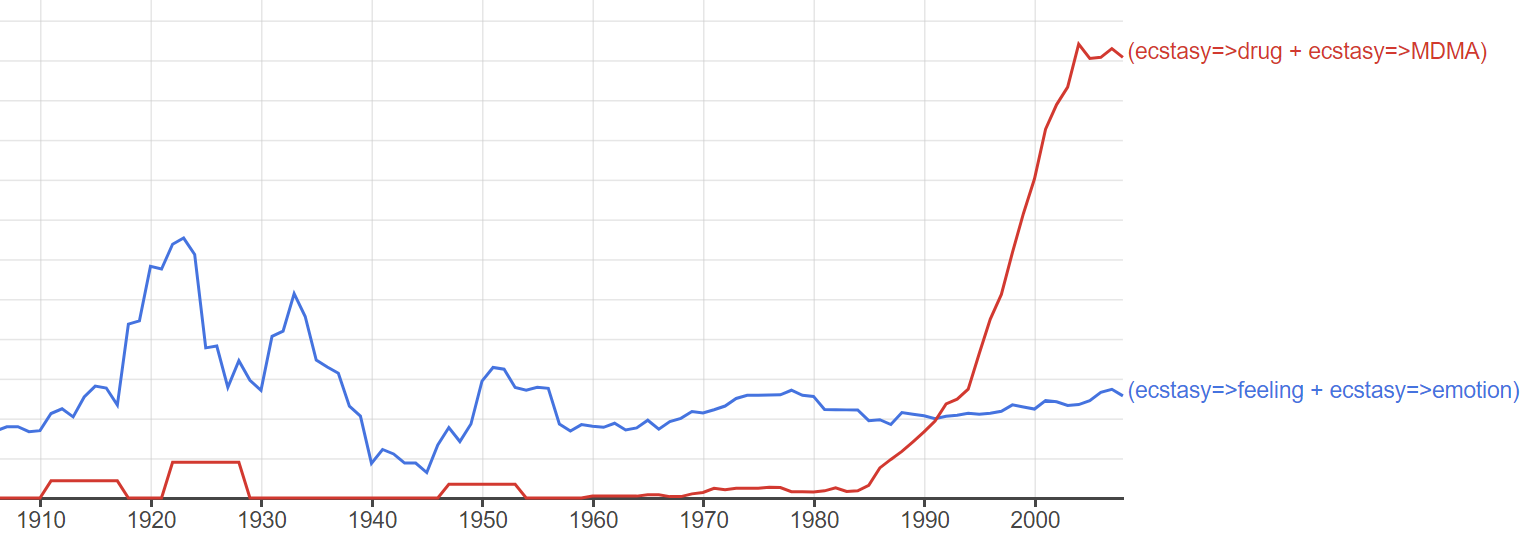
\includegraphics[width=\linewidth]{ecstasy_ngram.png}
	\caption{Google Ngram - ecstasy vs Ecstasy}
	\label{fig:ngram}
\end{figure}

One takes little comfort from the realization that the use of the word `ecstasy' has been trumped by a drug called Ecstasy that assists the user into a \emph{state of ecstasy}. This word ambiguation has an effect of diminishing the concept of emotional ecstasy in popular English language. When the reader hears the word `ecstasy' with minimal context on any given occasion, which occurrence comes to mind? Symbolic language is an imperfect tool.
 
This discussion can be confusing as it relies on subtle cultural inferences to make the point that many of the first wave anthropologists, scientists, and spiritual seekers who rediscovered existing drug ecstasy cultures or created the opportunity for entirely new ones in the laboratory, oft times reported regret for bringing casual public light to the heretofore unknown or forgotten substances. The frivolous, untrained, unserious use of mind-altering drugs, as expressed in pop culture, does encounter some risk. 


\subsection{psychedelic genesis}

The fascinating story of Gordon R Wasson tells of one such de facto anthropologist. A New York city banker by profession, Wasson was a pharmacological nonentity with no experience in chemistry or formal anthropology. In 1955 he and a photographer named Allan Richardson mounted a mission to the Mixeteco mountains of central Mexico to track down rumors of mystical mushrooms revealed in an obscure ten-year-old botanical journal.

There they met the Mixtec people and became the first white people in known history to participate in ceremonial consumption of \emph{divine} Psilocybe mushrooms. Wasson and his wife Valentina P Wasson, MD, would return each summer to the region, inquiring into the varieties of magic mushroom, and the rituals of their stewards.

In 1957, Life magazine published a multi-page article written by Gordon Wasson, detailing aspects of his experience. The article included several full-page photos and carefully drawn artwork depicting a variety of mushroom species. The article sparked tremendous interest in the funny `shrooms', inspiring a psychedelic tourism of hippies and beatniks seeking trippy times. The psychedelic revolution had begun. 

Sadly, the onslaught of questing visitors brought the attention of the Mexican police, threatening the Mixtec rituals and way of life. The medicine woman who originally shared her secrets with the Wassons was eventually ostracized from the community, and her house was raised, presumably by her people.

In roughly the same timeframe, the psychologist Humphrey Osmond had established a hallucinogenic drug study at the Weyburn Mental Hospital in Saskatchewan. Osmond had worked for a few years with mescaline and then transitioned to treating alcoholics with LSD. Of 2000 patients treated, Osmond reported that 40-45\% did not return to drinking after one year \cite{dyck_hitting_2006}.

Aldous Huxley, the British writer, known for the epically dystopian novel \emph{Brave New World}, had learned of mescaline and Dr. Osmond. He established a correspondence with Osmond, then, in 1953, Osmond introduced Huxley to the substance. \emph{The Doors of Perception} was published the following year; a 63-page philosophical essay detailing his trip.

In their subsequent friendship and correspondence, we witness the birth of the term psychedelic. Osmond instigated a dialog with the writer in search of a name for the effect of LSD on the mind. Huxley suggested \emph{phanerothyme}, from the Greek for ``to show'' and ``spirit,'' then promoted the term with a rhyme \enquote{To make this mundane world sublime, Take half a gram of phanerothyme.} Osmond countered with \emph{psychedelic}, from the Greek \emph{psyche} ``mind'' or ``soul'' and \emph{deloun}, ``show'', demonstrated in the shibboleth \enquote{To fathom Hell or soar angelic, Just take a pinch of psychedelic.} Osmond announced the new term at the 1957 New York Academy of Sciences meeting. 

\newpage

\begin{figure}[h!]
  \centering
  \begin{subfigure}[b]{0.4\linewidth}
    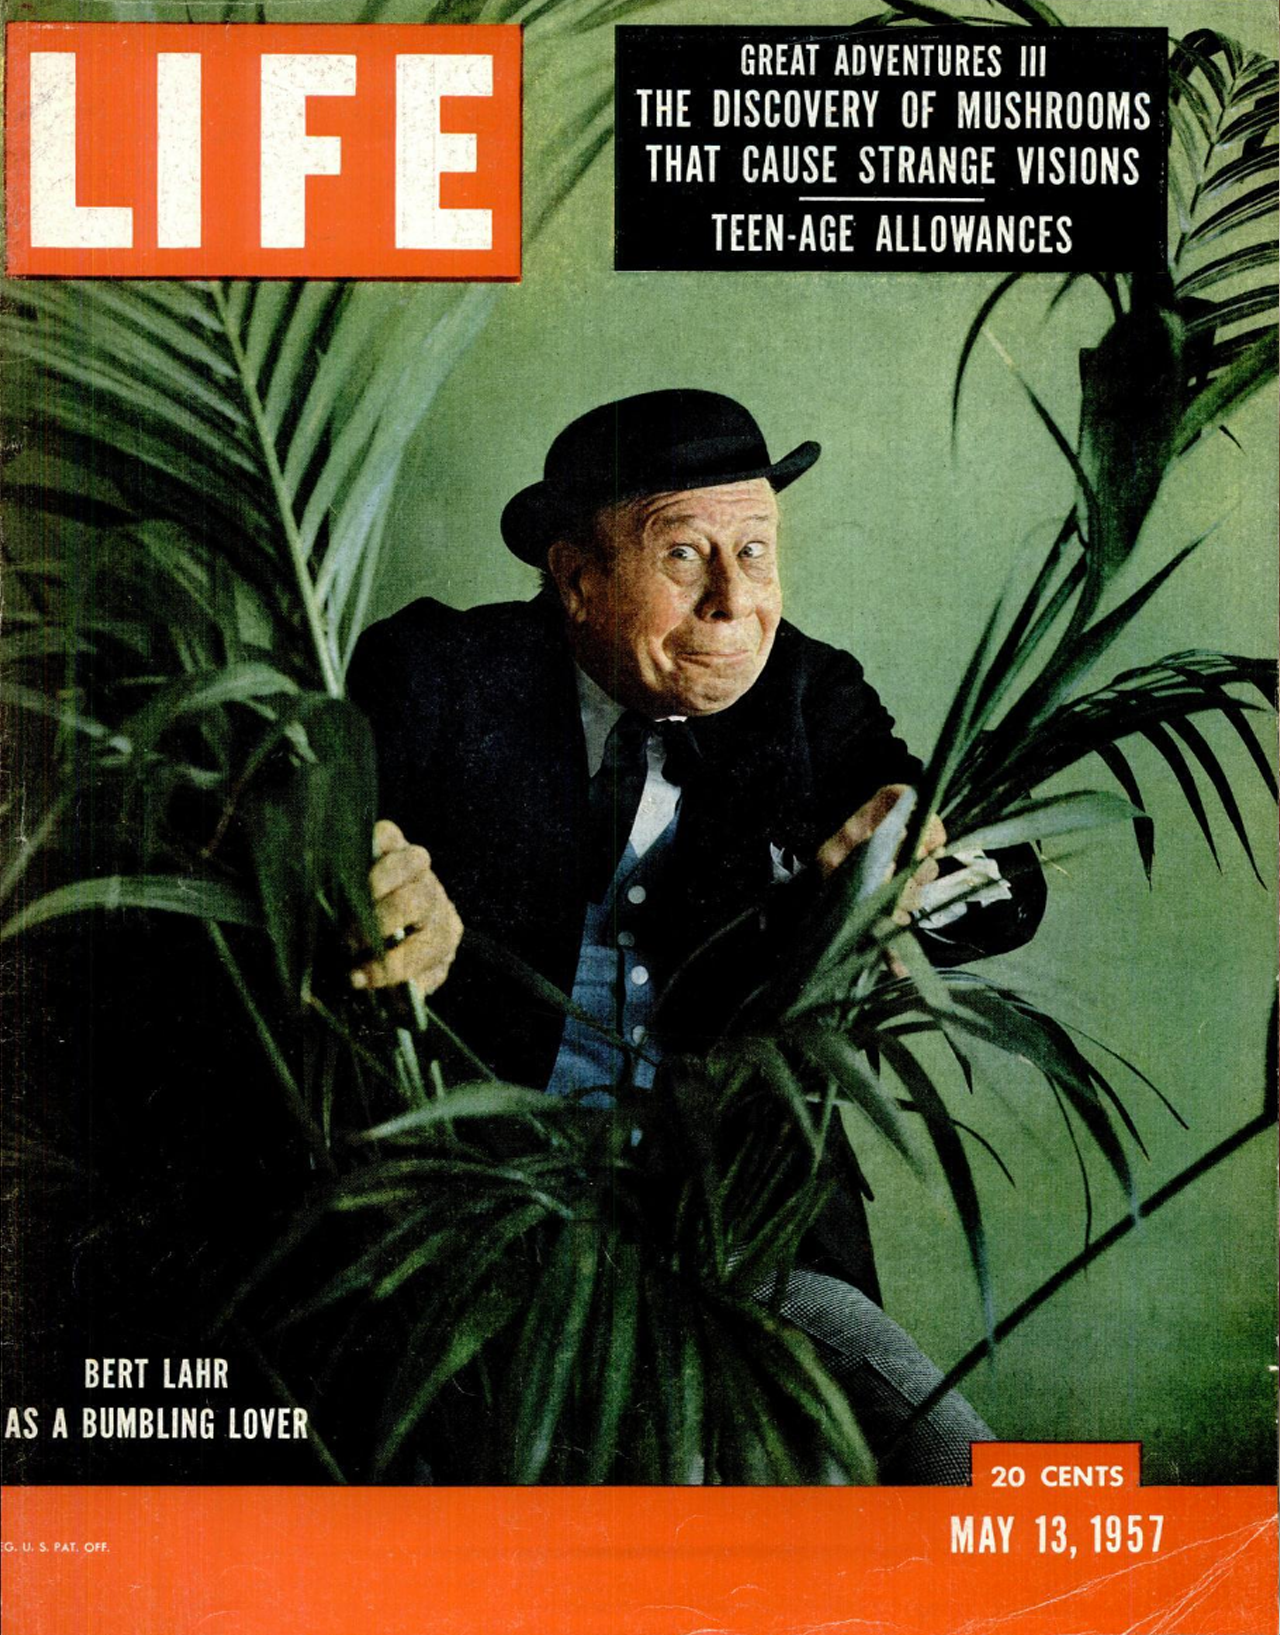
\includegraphics[width=\linewidth]{life57.png}
    \caption{Life 1957 - Seeking the Magic Mushroom}
  \end{subfigure}
  \begin{subfigure}[b]{0.4\linewidth}
    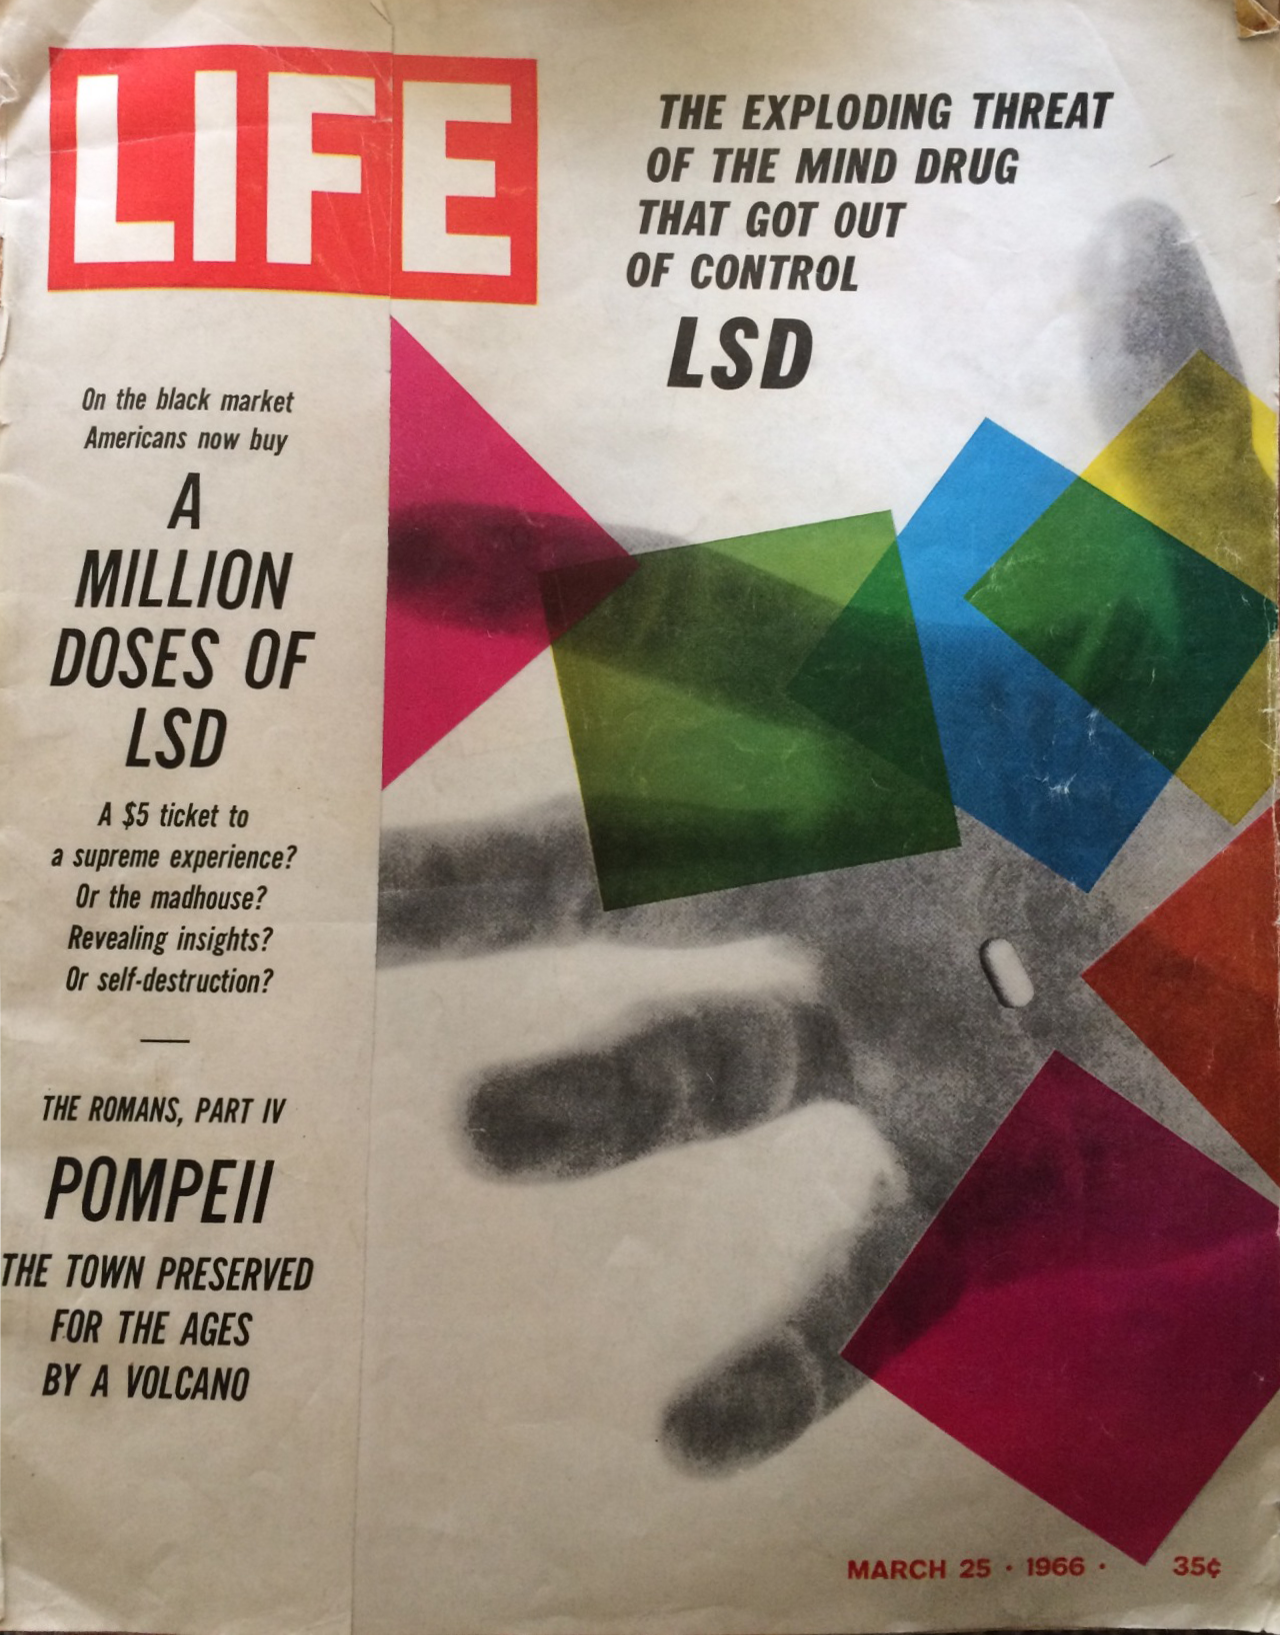
\includegraphics[width=\linewidth]{life66.png}
    \caption{Life 1966 - A Remarkable Mind Drug Suddenly Spells Danger}
  \end{subfigure}
  \caption{American's change of heart for psychedelics}
  \label{fig:hofmann}
\end{figure}

\subsection{psychedelic revolution}
\epigraph {Psychedelic drugs cause panic and temporary insanity---\\
in people who have not taken them!}{Timothy Leary 1963}

\vspace{9mm}

Wasson's article soon attracted the attention of a notable Harvard psychologist, Dr. Timothy Leary. A colleague, Anthony Russo, confirmed the veracity of the claims, having also made the journey to Mexico. In August of 1960, Russo accompanied Leary to Cuernavaca, Mexico, where he consumed psilocybin mushrooms for the first time. Of that first encounter, Leary is know to have said that he \enquote{learned more about\ldots (his) brain and its possibilities\ldots more about psychology in the five hours after taking these mushrooms than\ldots in the preceding 15 years of studying and doing research in psychology \cite{dassfierce}.} 

Within the year of his preeminent ecstatic psilocybin experience, Leary and his colleague Richard Alpert, together with board member Aldous Huxley, formed the Harvard Psilocybin Project, to document the effects of psilocybin on human consciousness. Recall that in that time, neither LSD nor psilocybin was classified substances. The team ordered psilocybin from the Sandoz lab, where Albert Hofmann had developed the process to derive the compound synthetically \cite{melechi_psychedelia_1997}.

With a steady supply of psychoactive potion on tap, Leary and Alpert administered the drug to volunteers from the Harvard student body, other researchers, prison inmates, and a group of divinity students. Of the last group, the famed ``Good Friday'' experiment, the Project researchers dosed the experimental group with psilocybin while attending a Good Friday service in a private chapel. The effect from the combined influence of intense religious ceremony and iconography, with psychoactive neurochemicals yielded a dramatic emotional response in the experimental group. Leary claimed that with entheogens \enquote{spiritual ecstasy, religious revelation, and union with God were now directly accessible \cite{mansnerus_timothy_1996}.}

Controversy followed the program in short order. The team's experiments suffered from unconventional design, such as non-random subject selection, and lacked proper control groups. More damning was the practice of the researchers taking the drugs themselves along with the subjects. Intradepartmental opponents of the project charged that the studies ``resembled cocktail parties,'' and that their data collection was sloppy.

The project ended in under three years. Harvard denied Leary a new contract after he failed teaching obligations, preferring to travel during that semester. Alpert was fired for giving drugs to undergrads, which was against the standing agreement with the school. Ultimately both were banned from academia. In short order, Alpert went to India to study at the Kainchi ashram, where he accepted a new name, Ram Dass, ``servant of God.'' Subsequently, he made a lifetime commitment to the spiritual path of non-exogenous self-induced ecstasy via disciplined meditation and yogic practice. He published a seminal yogi guidebook, Be Here Now, in 1971, often described as a countercultural bible. He continues to publish books and produce media content and events with the Be Here Now Network.

Leary followed a very different path, directing his attention to a pro-active mass counterculture of psychedelic non-conformity. In a prelude to the 1967 Summer of Love, 30,000 hippies gathered in Golden Gate Park, San Francisco, for the Human Be-In event. In a speech to the crowd, Leary delivered his now-famous phrase, ``Turn on, tune in, drop out.'' Leary claims that Marshall McLuhan crafted the phrase and had given it to him during a lunch meeting. McLuhan spoke about the marketing power of jingles and slogans and began singing a ditty to the melody of a popular Pepsi commercial that went something like,\enquote{Psychedelics hit the spot; Five hundred micrograms, that's a lot. Tune in, turn on, and drop out.}

Leary also popularized the phrase ``think for yourself and question authority,'' which he must surely have donned as a mantel, for over the two decades following his Harvard dismissal, he had been in dozens of jails on multiple continents, an escaped fugitive, and finally extradited from Afghanistan. Richard Nixon dubbed him ``the most dangerous man in America.'' Ironically, it was not yet illegal to possess his infamous drug of choice, LSD, but the marijuana tax act of 1937 had teeth. Of two minor marijuana arrests, one he successfully defended in the Supreme Court in 1969 for a clever technicality; the second landed him at Folsom Prison, where he served 5 of a 30-year sentence \cite{higgs_i_2006}.

By the mid-1960s, the tide had turned against the psychedelic tricksters. The nation was involved in a continuing unpopular armed conflict in Asia, and a de facto cultural war at home fueled by a youthful dissent. Nine years following Life's mischievous light-hearted 1957 magic mushroom article, a new ominous cover story read \enquote{The Exploding Threat of the Mind Drug That Got Out Of Control: LSD} with an overleaf addition that claimed \enquote{A Million Doses of LSD: \$5 ticket to a supreme experience? Or the madhouse? Revealing insights? Or self-destruction?} This was a verbose sign (1966 readers had perhaps less panache for zippy cover copy than today) that the establishment had become unsympathetic to the psychedelic credo. In 1970, LSD, psilocybin, mescaline, peyote, DMT, and chemicals resembling DMT, were added to the US Controlled Substance Act under Schedule I, followed in 1971 by the United Nations Convention on Psychotropic Substances. 

\newpage
\noindent

\includegraphics[width=\linewidth]{shaman_head.png}

\subsection{shamans}


The chilling effect of international embargo was hardly a new chapter. As we recall, it was only the cautious and nearly accidental discoveries of the early 20th century, from laboratory chemistry, to hobbyist anthropologists, they brought both synthetic and naturally-occurring consciousness-expanding substances into public awareness. 

\section{Ecstatic Novelty}


\subsection{subs}

% --------------------------------------------------------------------------
% -- CHAP 2 --
\chapter{Crossing Reality}
\label{Chapter:CrossingReality}
\epigraph {You are the universe experiencing itself.}{Alan Watts}

\vspace{9mm}

\section{Gathering the Senses}

\subsection{subs}

% --------------------------------------------------------------------------
% -- CHAP 3 --
\chapter{Building Reality}
\label{Chapter:BuildingReality}
\epigraph {A quote.}{Joe Blow}

\vspace{9mm}


\section{section}

\subsection{subs}

% --------------------------------------------------------------------------
% -- Summary and Conclusions --
\chapter{Summary and Conclusions}
\label{Chapter:SummaryAndConclusions}

Example summary and conclusions. You can refer to chapters and sections using their label, e.g Chapter \ref{Chapter:Introduction}.




% --------------------------------------------------------------------------
% -- References --

\clearpage
\renewcommand\bibname{References} % Relabels bibliography title as "REFERENCES"
\addcontentsline{toc}{chapter}{\textsc{\bibname}} % Adds to table of contents
\bibliographystyle{plain}  % Sets style, plain is fine for this
\bibliography{exr-unk}  % Name of bibliography file containing your references. It is best practice to have a separate file, as it makes it easier to share your references, make derivative works, or use the references from a prior work (e.g a prior paper that your thesis work is building on).

% Examples of citing GitHub repositories:
%   http://academia.stackexchange.com/a/14015
%   https://github.com/blog/1840-improving-github-for-science
%   https://guides.github.com/activities/citable-code/
%   https://github.com/GhostofGoes/uidaho-masters-thesis/
%   Wait, that last one is recursive...oh no. RIP poorly programmed web crawling spider.




% --------------------------------------------------------------------------
% -- Appendices --
\clearpage
\appendix  % Marks start of appendices

% Appendices are done as LaTeX chapters
\chapter{Your fist appendix}
First appendix content

% ** This is an example of a YAML file listing, but it could be anythig, e.g full experiment results, or list of equipment used. **
% \clearpage
% \chapter{Exercise Specification}
% \lstinputlisting[firstline=56, firstnumber=1, language=yaml,caption=Exercise Specification]{Specifications/exercise-specification.yaml}

% ** Example of a Python script code listing **
% \clearpage
% \chapter{vsphere-info Script Source Code}
% \lstinputlisting[firstline=16, firstnumber=1, language=python, caption=vsphere-info script]{Code/scripts/vsphere_info.py}



\end{document}

% ** DO NOT PUT ANYTHING AFTER THE END OF THE DOCUMENT! **
